\documentclass{standalone}

\usepackage{tikz}
\usetikzlibrary{matrix}

\newcommand{\lra}{\longrightarrow}

\begin{document}
\renewcommand*{\arraystretch}{2}
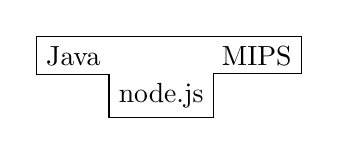
\begin{tikzpicture}

	\matrix(m)[matrix of nodes]{
			Java  		&&  MIPS	\\
			& node.js	&   		\\
	};

	\draw (m-1-1.south west) |- (m-1-3.north east) |- (m-2-2.north east) |- (m-2-2.south west) |- (m-1-1.south west);

\end{tikzpicture}

\end{document}
